\documentclass{article}
\usepackage{graphicx} % Required for inserting images
\usepackage[top=0.9in, bottom=1in, left=1.5in, right=1.5in]{geometry}
\usepackage[utf8]{inputenc}
\usepackage[icelandic]{babel}
\usepackage[T1]{fontenc}
\usepackage[sc]{mathpazo}
\usepackage[parfill]{parskip}
\renewcommand{\baselinestretch}{1.2}
\usepackage{booktabs,tabularx}
\usepackage{multirow}
\usepackage{enumerate}
\usepackage{adjustbox}
\usepackage{multicol}
\usepackage{xcolor}
\usepackage{algpseudocode}
\usepackage{tikz}
\usepackage{nicefrac}
\usepackage{changepage}
\usetikzlibrary{arrows, positioning, calc, graphs}
\usepackage{amsmath, amsfonts, amssymb, amsthm}
\usepackage{graphicx}
\usepackage{tikz}
\usepackage{minted}
\usemintedstyle{manni}
\title{Tölvutækni og Forritun Heimadæmi 9 }
\author{Ragnar Björn Ingvarsson, rbi3}
\tikzset{->, >=stealth', shorten >=1pt, node distance=2cm,thick, main node/.style={circle,draw,minimum size=3em}}

\begin{document}
\renewcommand\thepage{}

	\maketitle

	\newpage
	\setcounter{page}{1}
	\renewcommand\thepage{\arabic{page}}

	\section{}
	\begin{itemize}
		\item[a)] Veljum 12 TB Seagate IronWolf sem stóra diskinn okkar og 
			4 TB Western Digital Purple sem litla. Stóri kostar $49900$ en 
			litli $19500$. Þá fæst að verð/TB fyrir stóra er:
			\begin{equation}
				49900/12 \approx 4158\text{ kr/TB}
				\label{eq:gamer}
			\end{equation}
			En fyrir litla:
			\begin{equation}
				19500/4 = 4875\text{ kr/TB}
				\label{eq:gamer1}
			\end{equation}
		\item[b)] Tökum 4 TB Samsung 870 QVO sem stóra og 500 GB Samsung 
			870 EVO sem litla og fáum fyrir stóra:
			\begin{equation}
				46900/4 = 11725\text{ kr/TB}
				\label{eq:gamer2}
			\end{equation}
			Og fyrir litla:
			\begin{equation}
				10500/0.5 = 21000\text{ kr/TB}
				\label{eq:gamer3}
			\end{equation}
		\item[c)] Aðalástæður fyrir áframhaldinni notkun seguldiska er bæði 
			lágt verð þeirra, sem mun haldast á næstu árum sem fimmfalt 
			minna heldur en storkudiskar og einnig að seguldiskar eru 
			miklu betur aðlagaðir fyrir stóra geymslu gagna, sérstaklega 
			fyrir svokölluð köld gögn, sem eru ekki oft notuð og ætluð 
			helst til geymslu til framtíðar.

			Þannig að storkudiskar og seguldiskar munu haldast í jafnvægi 
			þar sem storkudiskar munu aðallega vera notaðir fyrir staði þar 
			sem mikið þarf að flytja gögn en seguldiskar munu halda áfram 
			að vera notaðir í geymslu gagna.
	\end{itemize}

	\section{}
	\begin{itemize}
		\item[i. \& ii.] 
			Innsetningarröðun er með fína staðværni í bæði 
			tíma og rúmi þar sem þegar búið er að raða staki er mjög líklegt 
			að það þurfi að fá aðgang að því aftur til að bera saman við 
			næsta stak, og einnig, þar sem röðunin inn í raðaða listann 
			er aðalparturinn af reikniritinu, er oftast verið að ná í 
			stök sem eru við hlið hvors annars.

			Quicksort er með góða staðværni í rúmi þar sem þegar verið er 
			að skipta fylkinu þarf að fara í gegn um hvert stak eitt í einu, 
			og einnig, þar sem verið er að skipta í litla hópa í raun, 
			þá eru stök mikið notuð saman innan síns hóps. Hins vegar held 
			ég að quicksort sé ekki með mjög góða staðværni þegar það kemur 
			að tíma þar sem alltaf er verið að hoppa frá hópi til hópar 
			og stök eru ekkert endilega alltaf notuð mjög oft í röð.

			Þess vegna tel ég innsetningarröðun betri þegar kemur að 
			staðværni.
	\end{itemize}

	\newpage
	\section{}
	\begin{itemize}
		\item[a)] Súluritið sem fæst lítur svona út
			\begin{center}
				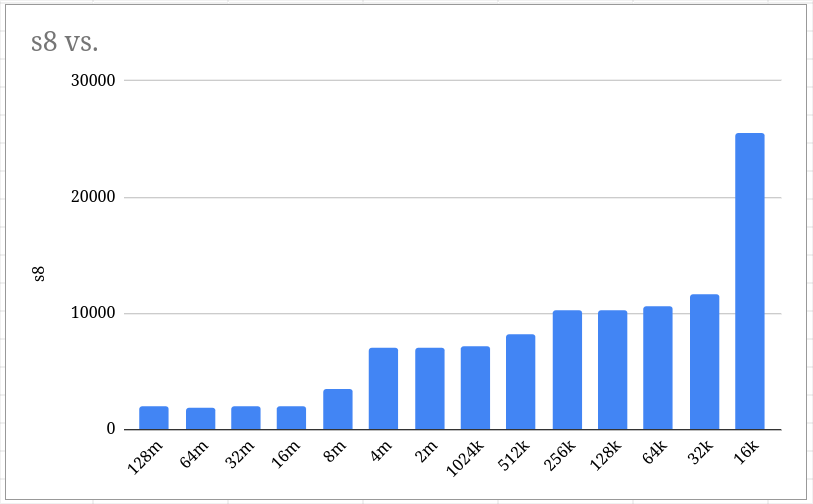
\includegraphics[scale=0.35]{s8.png}
			\end{center}
			Og útfrá því er hægt að lesa að fyrst mikið fall er frá 16k yfir 
			í 32k þá er L1 líklegast 16k, sama gengur með frá 256k yfir 
			í 512k svo L2 er líklegast 256k, og svo loks er L3 líklega 
			4m þar sem eftir það í 8k lækka lestrarafköstin enn meira.
		\item[b)] Súluritið hér kemur út sem
			\begin{center}
				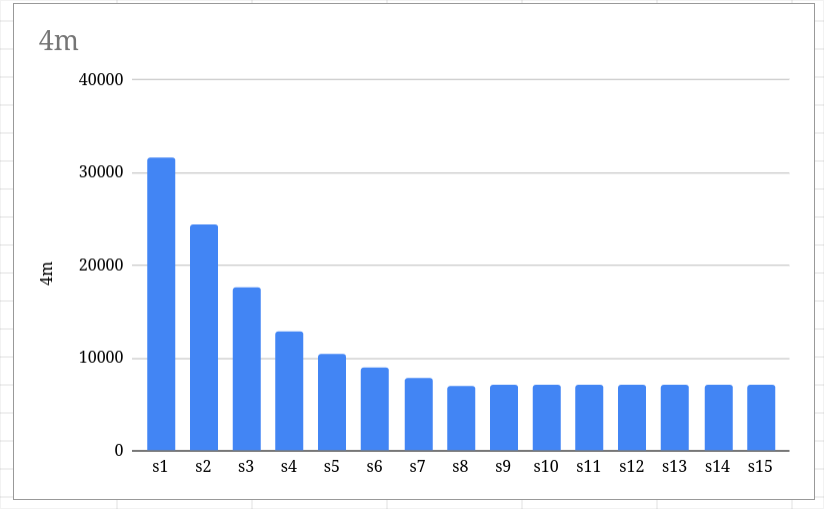
\includegraphics[scale=0.35]{4m.png}
			\end{center}
			Og útfrá þessu er hægt að lesa að um skrefstærð 8 jafnast 
			út afköstin, svo líklega nær L2 bara upp í skrefstærð $8$, 
			sem er þá $\frac{4096}{8\cdot8} = 64$ bæti.
		\item[c)] Til að finna líklega línustærð L1 er örugglega best að 
			nota þá 256k vinnumengi þar sem þá erum við á enda þess sem L1 
			getur höndlað.
			\begin{center}
				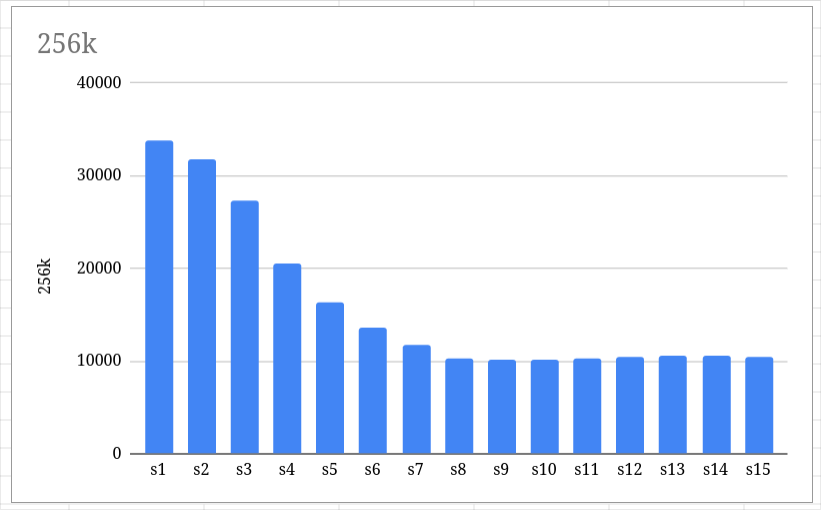
\includegraphics[scale=0.35]{256.png}
			\end{center}
			Þá kemur svona súlurit og við sjáum hér að allt verður flatt 
			um s8, svo línustærð af $\frac{256}{8\cdot8} = 4$ bæti.
	\end{itemize}

	\section{}
	\begin{itemize}
		\item[a)] Við erum með heildarstærð $2048$ bæti sem er dreift 
			niður á línur með $16$ bæti hvert, og hvert mengi er þá með 
			$2$ línur hvert, svo fjöldi mengja er
			\begin{equation}
				\frac{2048}{16\cdot2} = 64
				\label{eq:gamer4}
			\end{equation}
		\item[b)] Vitum að bitunum er skipt í merki, mengisnúmer og 
			blokkarhliðrun, og við vitum að blokkarhliðrunin verður að hafa 
			pláss til að sýna $16$ möguleika, svo $4$ bita, mengisnúmerið 
			er þá $6$ bitar þar sem þá getum við sýnt $64$ möguleika, svo 
			merkið fær rest sem er þá $16 - 6 - 4 = 6$ bitar.
	\end{itemize}

	\section{}
	\begin{itemize}
		\item[a)] Erum þá með heildarstærð $4$KB og $128$ bæta línustærð 
			og $4$-vítt minni svo hvert mengi er $128\cdot4 = 512$ bæti, 
			og þá eru $\nicefrac{4096}{512} = 8$ mengi.
		\item[b)] Við sjáum að þar sem hvert mengi er $512$ bæti og 
			línustærðin er $128$ bæti þá eru $\frac{512}{128} = 4$ ólíkar 
			línur sem varpast í sama mengi.
		\item[c)] Sjáum að við þurfum þrjá bita fyrir mengisnúmer, 
			$7$ fyrir blokkarhliðrun og þá bara $10$ fyrir merkið. Þá erum 
			við með efsta bitann af $2$ og neðstu tvo af $3$ fyrir 
			mengisnúmerið sem gefur $110_2$ svo mengi $6$.
		\item[d)] Sjáum að mengisnúmer og blokkarhliðrun taka samanlagt $10$ 
			bita, svo merki tekur rest, þ.e. $0101010000_2$, þannig að 
			t.d. \texttt{0x54231} virkar og varpast ekki í sama mengi.
	\end{itemize}
\end{document}
